%%%%%%%%%%%%%%%%%%%%%%%%%%%%%%%%%%%%%%%%%%%%%%%%%%%%%%%%%%%%%%%%%%%%%%%%%%%%%%%%%%%%%%%%%%%%%
%%%%%%%%    CS437/CS5317/EE414/EE513 -- Deep Learning, Spring 2026, LUMS              %%%%%%%%
%%%%%%%%    Final Project Report -- Group 4                                           %%%%%%%%
%%%%%%%%    Built on the modified ICML 2021 template provided in class.               %%%%%%%%
%%%%%%%%%%%%%%%%%%%%%%%%%%%%%%%%%%%%%%%%%%%%%%%%%%%%%%%%%%%%%%%%%%%%%%%%%%%%%%%%%%%%%%%%%%%%%

\documentclass{article}

\usepackage{microtype}
\usepackage{graphicx}
\usepackage{subfigure}
\usepackage{booktabs}
\usepackage{amsmath}
\usepackage{amssymb}
\usepackage{bm}
\usepackage{multirow}
\usepackage{xcolor}
\usepackage{url}

\usepackage{hyperref}
\hypersetup{
    colorlinks=true,
    linkcolor=black,
    citecolor=black,
    urlcolor=blue
}

\newcommand{\theHalgorithm}{\arabic{algorithm}}

\usepackage[accepted]{icml2021}

\icmltitlerunning{YOLO+CLIP for Forest Fire Detection}

\begin{document}

\twocolumn[
\icmltitle{Reducing False Positives in Real-Time Forest Fire and Smoke Detection
           via Cascaded Vision-Language Verification}

\begin{icmlauthorlist}
\icmlauthor{Muhammad Baqir Hassan Babar (27100340)}{}
\icmlauthor{Momin Fahed Khan (27100082)}{}
\end{icmlauthorlist}

\icmlkeywords{forest fire detection, YOLO, CLIP, semantic verification, false positive reduction}

% Force the running header (ICML 2021's auto-check rejects the long title even
% with \icmltitlerunning supplied, so we set \chead explicitly).
\chead{\small\bf YOLO+CLIP for Forest Fire Detection}

\vskip 0.15in

{\centering
\textbf{Group 4} $\;\cdot\;$ CS437/CS5317/EE414/EE513 --- Deep Learning, Spring 2026, LUMS\\[2pt]
\textbf{Code:} \url{https://github.com/27100340/dl-forest-fire-detection.git}\par}
\vskip 0.20in
]

% =============================================================================
\begin{abstract}
Real-time forest fire detection from PTZ camera feeds is dominated by a single
failure mode: detectors confidently fire on fog, clouds, haze, sun glare, and
lamp lights because those patterns visually resemble fire and smoke. We
investigate whether a lightweight \emph{semantic verification} stage attached
to a YOLOv8n detector can suppress these false positives without sacrificing
the recall that makes the detector useful. We build three systems on the D-Fire
benchmark. The baseline YOLOv8n reaches 76.1\% mAP@0.5 with a 2.44\%
hard-negative false positive rate (FPR). Our first improvement adds a
zero-shot CLIP verifier with a confounder-aware prompt bank; this cuts
hard-negative FPR to 0.55\% (a 77\% relative reduction) but causes a 22.6
percentage-point drop in mean recall because internet-trained CLIP rejects
genuine forest-domain smoke as ``fog''. Our second improvement replaces the
zero-shot prompt bank with a logistic-regression linear probe trained on
CLIP features of D-Fire crops, with hard-negative crops mined from YOLO's own
false positives and 12 confounder text prompts injected as synthetic negatives
in feature space. The probe brings hard-negative FPR down to 0.70\% (a 71\%
relative reduction over baseline) while recovering recall to within 4.4
percentage points of the YOLO-only system, at 21\,ms mean latency on a Tesla T4
--- well under the 100\,ms edge-deployment budget. The headline finding is that
the appropriate role for CLIP in fire detection is not zero-shot
classification but as a frozen feature extractor for a domain-adapted probe.
\end{abstract}

% =============================================================================
\section{Introduction}
\label{sec:intro}

Forest fires destroy millions of hectares of land each year and are responsible
for substantial loss of life, property, and biodiversity. Suppression cost
scales nonlinearly with how long a fire burns before detection, so any reduction
in detection latency is directly load-bearing for deployment value. Networks of
Pan-Tilt-Zoom (PTZ) cameras --- such as those operated by the World Wide Fund
for Nature (WWF) in our deployment scenario --- offer continuous visual coverage,
but human operators cannot watch every feed in real time. The bottleneck has
shifted from the sensor to the inference layer: we need a detector that runs in
real time on edge hardware, finds genuine smoke and fire while it is still
small, and \emph{does not page operators on every fog bank, sunlit cloud, or
streetlight in view}.

Off-the-shelf object detectors solve part of the problem. Recent YOLO variants
deliver $>$30\,FPS on Jetson-class hardware and routinely report 70--85\%
mAP@0.5 on fire benchmarks. They are, however, also routinely reported as
producing false alarms in numbers that would make any deployed system
unusable: a single PTZ camera capturing fog at sunrise can trigger dozens of
spurious alerts before lunch. Across the survey we conducted in
Deliverable~1 (12~papers), the gap that recurs is the same: every method
treats fire and smoke detection as pure visual pattern matching, and none has a
mechanism for asking ``does this region's broader visual context look like
smoke, or like fog?''.

We explore a hypothesis suggested but never tested in that literature: a frozen
CLIP~\cite{clip} encoder, applied only to the cropped regions a YOLO detector
has already proposed, can serve as a low-cost semantic discriminator. The
proposed pipeline is a cascade in the classical sense --- the expensive verifier
sees only what the cheap detector flags --- so the latency overhead is bounded
by the number of detections per frame, not the resolution of the input.

Our work proceeds in three stages, each with experimental commitments.

\textbf{Baseline (Section~\ref{sec:baseline}).} Fine-tune YOLOv8n on D-Fire and
characterise the failure mode quantitatively. We establish that the
hard-negative false positive rate, not the mAP, is the deployment-blocking
metric.

\textbf{Improvement~1 (Section~\ref{sec:i1}).} Add a zero-shot CLIP verifier
with a 22-prompt bank that names confounders explicitly. We measure how much
of the FPR is the visual-similarity problem the literature describes, and how
much is the hardness of the underlying detector's mistakes.

\textbf{Improvement~2 (Section~\ref{sec:i2}).} Replace the zero-shot prompts
with a supervised linear probe over the same CLIP features, trained on D-Fire
crops with aggressive hard-negative mining and text-anchored synthetic
negatives. We add a confidence-gated cascade so that high-confidence YOLO
detections bypass the verifier entirely.

The contribution of this work is the empirical finding that the bottleneck in
the YOLO+CLIP family is the verifier, not the detector, and that the right
intervention is a domain-adapted probe over frozen CLIP features rather than
either retraining the detector or replacing the prompt bank. We show this on
the D-Fire benchmark across the standard set of metrics, with a Pareto-style
operating-point analysis that makes the precision/recall trade-off explicit.

% =============================================================================
\section{Related Work}
\label{sec:related}

We summarise the related-work analysis from our SOA survey~(Deliverable~1)
along the three challenges that organise the literature.

\paragraph{C1. Smoke versus visually similar phenomena.}
Every reviewed system documents false positives from fog, clouds, haze, sun
glare, and reflective surfaces. Li and Zhao~\cite{cnn_fire_detection}
benchmarked Faster~R-CNN, R-FCN, SSD, and YOLOv3 on a custom fire dataset whose
annotation schema explicitly tags ``disturbance'' objects (fire-like and
smoke-like non-fire elements); even their best detector (YOLOv3, 83.7\% mAP
at 28\,FPS) confidently fires on those disturbances. Abdusalomov
et al.~\cite{detectron2fire} reach 99.3\% precision with Detectron2 and
Mask~R-CNN, but only after augmenting with 13{,}800 sunlight images, identifying
sunlight as their single largest false-positive driver. Zheng
et al.~\cite{cnn_vit_smoke} hybridise CNNs with a Vision Transformer
(SR-Net) for satellite imagery and report a Grad-CAM analysis showing that the
network's attention drifts off smoke when point-like clouds enter the scene.
Zhao et al.~\cite{spectral_smoke} attack the smoke--cloud confusion in the
spectral domain (multi-band Landsat) but cannot generalise to RGB-only PTZ
sensors. None of these works contains a semantic-reasoning layer.

\paragraph{C2. Real-time inference under edge constraints.}
A 100\,ms-per-frame budget on Jetson-class hardware is the practical
ceiling for PTZ deployment. YOLOv3~\cite{cnn_fire_detection} and
YOLOv8~\cite{yolov8_smartcity} clear it; two-stage detectors such as
Mask~R-CNN do not~\cite{detectron2fire}. The architectural insight that
motivates our cascade is that the verifier does not need to process the whole
frame --- only the boxes the detector has already produced. CLIP ViT-B/32 over
$\sim$5--10 cropped patches at 224$\times$224 is cheap relative to a
640$\times$640 second-stage detector.

\paragraph{C3. Early-stage smoke with weak visual cues.}
Cao et al.~\cite{bilstm_smoke} use BiLSTM with temporal attention over PTZ
patch sequences to reach 97.8\% accuracy on a forest-smoke dataset --- but their
output is a frame-level classification, not boxes, and their method requires
multiple temporally adjacent frames. FireMatch~\cite{firematch} uses semi-
supervised learning to combat label scarcity, but explicitly notes that
``confusing samples'' (strong lights, moving smoke) remain a primary failure
mode. The IoT-based system of~\cite{iot_nodefire} reduces false alarms by
fusing temperature and humidity sensors --- a multi-modal principle whose
vision-only analog is precisely what a CLIP verifier provides.

\paragraph{The unaddressed gap.}
Every surveyed work treats detection as pixel-level pattern matching. None
incorporates a vision-language model for semantic verification despite CLIP's
established zero-shot performance on natural-image categories~\cite{clip}.
The closest spirit-aligned work, SR-Net~\cite{cnn_vit_smoke}, hybridises a
CNN with a Vision Transformer~\cite{vit} \emph{end-to-end} rather than as a
post-hoc verifier --- so the transformer attends to the same features as the
backbone and inherits its blind spots. Our project tests whether plugging a
frozen, internet-pretrained vision-language model into the cascade --- as an
explicitly orthogonal perceptual prior --- can break the FPR bottleneck.

% =============================================================================
\section{Methodology}
\label{sec:method}

We share the dataset, the baseline weights, and the YOLO inference settings
across all three systems described below. Differences live entirely in the
verifier.

\subsection{Dataset}
\label{sec:dataset}

We use the D-Fire benchmark of de Ven\^{a}ncio
et al.~\cite{dfire_dataset}: 21{,}527 RGB images with YOLO-format bounding
boxes for two classes (\texttt{0=smoke}, \texttt{1=fire}). Empty label files
denote \emph{hard-negative} images that contain confounders such as fog, sun
glare, lamp lights, and reflective surfaces. The split sizes are
14{,}122/3{,}099/4{,}306 (train/val/test) of which the test split contains
2{,}005 hard-negative images --- this is the subset on which we report FPR.
This is the same D-Fire mount used across Deliverables~3, 4, and 5 (Kaggle
slug \texttt{sayedgamal99/smoke-fire-detection-yolo}).

\subsection{Baseline: YOLOv8n}
\label{sec:baseline}

The baseline is YOLOv8n initialised from COCO weights and fine-tuned on
D-Fire for 50 epochs at imgsz~640 with batch size 16, optimiser \texttt{auto}
(SGD), $\text{lr}_0{=}0.01$, mosaic 1.0, fliplr 0.5, patience 10,
\texttt{close\_mosaic}~10, and seed 42. Training was performed on a single
Tesla T4 (Kaggle).

YOLOv8n was chosen, rather than a larger variant, for two reasons. First, the
n-variant is the only YOLOv8 size that comfortably meets a 100\,ms latency
budget after a verifier stage is added. Second, the gap we want to attack is
recall vs.\ FPR on confounders --- a problem that scaling the detector does not
fix in the surveyed literature, so a stronger backbone would not help us
isolate the verifier's contribution. We freeze these weights for all
subsequent improvements.

\subsection{Improvement 1: Zero-shot CLIP semantic verifier}
\label{sec:i1}

The first improvement adds a CLIP ViT-B/32~\cite{clip} verifier between YOLO
and the final accept/reject decision. For each YOLO detection at conf $\geq$ 0.25,
we expand the box by a 20\% margin, crop, encode with the CLIP image encoder,
and compute cosine similarity to a precomputed bank of 22 text prompts:

\begin{itemize}\itemsep1pt
\item \textbf{Fire (5):} ``a photo of fire'', ``a photo of flames burning'',
      ``a photo of a forest fire'', ``a photo of a wildfire with visible
      flames'', ``a close-up photo of orange burning flames''.
\item \textbf{Smoke (5):} ``a photo of smoke'', ``a photo of a smoke plume
      rising'', ``a photo of thick smoke from a fire'', ``a photo of grey smoke
      in a forest'', ``a photo of smoke from burning trees''.
\item \textbf{Confounders (12):} fog, mist, clouds, haze, cloudy sky, sunlight,
      sun glare, lamp/streetlight, reflective surface, normal forest, fire-truck
      lights, sunset --- naming the confounders explicitly is critical, as the
      ablation in Section~\ref{sec:results} shows.
\end{itemize}

The decision rule is a bucketed argmax: we group the 22 prompts into three
buckets (fire / smoke / confounder), assign the crop to the bucket containing
its top-similarity prompt, and \emph{keep} the YOLO detection iff its top
bucket matches the YOLO class label. This realises the SOA's stated research
question --- ``does this region semantically look more like smoke than fog?'' ---
without any training on D-Fire.

\subsection{Improvement 2: CLIP linear probe with cascaded gating}
\label{sec:i2}

Improvement~1's recall collapse (Section~\ref{sec:results}) signalled that
zero-shot CLIP, although strong as a confounder rejector, was rejecting
forest-domain smoke too. Smoke in PTZ imagery is faint and diffuse; CLIP, trained
on internet-scale image-text pairs, overweighs the visual similarity to its
``fog''/``haze'' prompts and votes wrong on a substantial fraction of true
smoke. Improvement~2 replaces the prompt-based decision rule with a
supervised classifier over the same CLIP features, while keeping the rest of
the pipeline identical.

\paragraph{Architecture.} The cascade has two stages and one shortcut.
\textbf{(i) Detection.} YOLOv8n produces boxes with class and
confidence. Detections at conf $\geq \tau_{\text{high}}$ (default 0.7) are
\emph{auto-kept} and skip the verifier; this preserves recall on easy-positive
cases that do not need a second opinion. \textbf{(ii) Cropping.} For each
remaining detection we extract a 20\%-margin crop and encode it with frozen
CLIP ViT-B/32 (512-dim L2-normalised features). \textbf{(iii) Probe.} A
3-class logistic-regression head ($\text{smoke}/\text{fire}/\text{neg}$)
predicts the crop label; we keep the detection iff the probe's argmax matches
the YOLO class.

\paragraph{Probe training data.} The probe is trained \emph{only} on
crops drawn from the D-Fire training split, never from validation or test.
We assemble three sources.

\textit{Positive crops:} every ground-truth fire/smoke box in the train split,
expanded by the 20\% margin, encoded with CLIP. This yields 7{,}788 smoke and
9{,}629 fire crops.

\textit{Mined hard negatives:} we run the frozen YOLO at a low confidence
threshold (conf~$=$~0.03) on every train-split \emph{negative} image (empty
labels) and every val-split negative image. Because these images contain no
fire and no smoke by definition, every detection is by construction a false
positive --- the exact distribution of confounder crops we want the probe to
reject. This produces 1{,}071 hard-mined negative crops (vs.\ 282 at
conf~$=$~0.10 in our v1 probe; we found that the more aggressive threshold
materially improved coverage).

\textit{Text-anchored synthetic negatives:} the 12 confounder text prompts
from Improvement~1 already live in CLIP's joint image-text feature space.
We encode each, perturb with small isotropic Gaussian noise
($\sigma{=}0.02$), L2-renormalise, and replicate 50 times --- producing 600
synthetic negative features that anchor the probe's decision boundary near
explicit confounder concepts (``fog'', ``cloud'', ``sun glare'', $\dots$).
This is a cheap way to inject Improvement~1's prior into Improvement~2's
classifier without re-introducing zero-shot's failure mode.

\textit{Random negatives:} 500 random patches from train-split negative
images (capped down from 5{,}000 in our v1 probe; we found that excess random
negatives diluted the mined+anchored signal).

\paragraph{Probe.} A 3-class multinomial logistic regression with
\texttt{class\_weight='balanced'}, \texttt{C=10}, \texttt{lbfgs} solver,
fit in $\sim$5\,s on $\sim$20\,k examples. It is small enough to never overfit
a 512-dimensional space --- 5-fold sanity-check accuracy on a held-out 10\%
slice of the training crops is 87.9\%. We compared against a 1-layer
64-unit MLP probe (40 epochs, dropout 0.2, weight decay $10^{-4}$); on
deployment metrics the two are statistically identical
(Section~\ref{sec:results}).

\paragraph{Inference cost.} The probe is $512\times3$ matrix-vector multiply
plus a softmax --- microseconds. The dominant cost remains the CLIP image
encoder. We expect Improvement~2 to be no slower than Improvement~1; we
verify this in Section~\ref{sec:results}.

% =============================================================================
\section{Experiments and Results}
\label{sec:results}

We report all numbers on the held-out D-Fire test split (4{,}306 images), with
hard-negative FPR computed on the 2{,}005-image hard-negative subset. Two
evaluation harnesses are used. The first is Ultralytics' native
\texttt{yolo.val()}; this gives the canonical baseline mAP@0.5~$=$~0.7614
that we cite in the abstract. The second is a custom IoU-matched
greedy-AP harness (11-point AP, IoU~$=$~0.5, class-conditional matcher) that
runs inside Improvement~2's notebook over both Improvement~1 and Improvement~2;
this harness is what we use for \emph{cross-system} comparisons because the
native evaluator is not aware of a downstream filter and would silently produce
inconsistent numbers across systems. See the GitHub repository for both
implementations and a side-by-side justification.

\subsection{Headline result --- Pareto frontier on FPR vs.\ recall}

Table~\ref{tab:headline} summarises the comparison across all five systems:
the YOLO-only baseline (both harnesses), Improvement~1, Improvement~2's
default probe (v1), our headline probe with aggressive negative mining and
text anchors (v2), and an additional ensemble that ANDs the v2 probe with
Improvement~1's text-prompt argmax. The same numbers are plotted as a
trade-off scatter in Figure~\ref{fig:frontier}.

\begin{table*}[t]
\caption{Headline results on the D-Fire test set. Cascade rows are produced
by the same custom evaluation harness (custom 11-point AP, greedy class-
conditional IoU=0.5 matcher) so that I1, I2, and the YOLO-only reference are
apples-to-apples. ``Native YOLO'' is the canonical Ultralytics
\texttt{yolo.val()} number. HN-FPR is image-level false-positive rate on the
2{,}005 hard-negative test images. Best in column \textbf{bold}.}
\label{tab:headline}
\vskip 0.10in
\begin{center}
\begin{small}
\begin{tabular}{lcccccc}
\toprule
\textbf{System} & \textbf{mAP@0.5} & \textbf{Mean P} & \textbf{Mean R} & \textbf{HN-FPR} & \textbf{Latency (ms)} & \textbf{$\Delta$ vs.\ YOLO} \\
\midrule
Native YOLO (yolo.val)              & \textbf{0.7614} & \textbf{0.7696} & 0.6971       & 2.44\% & 16.5 & --- \\
YOLO-only (custom harness)          & 0.6370          & 0.7481          & \textbf{0.7272} & 2.44\% & \textbf{13.2} & --- \\
\midrule
I1 -- zero-shot CLIP                & 0.5559          & 0.8091          & 0.5625       & 0.55\% & 20.8 & FPR $-77\%$, R $-23$\,pp \\
I2 -- LR probe v1                   & 0.6365          & 0.7649          & 0.7029       & 1.25\% & 21.2 & FPR $-49\%$, R $-3$\,pp \\
\textbf{I2 -- LR probe v2 (ours)}   & 0.6355          & 0.7714          & 0.6830       & \textbf{0.70\%} & 21.1 & FPR $\bm{-71\%}$, R $-4$\,pp \\
I2 -- ensemble (v2 + text)          & 0.5576          & 0.7968          & 0.6063       & \textbf{0.30\%} & 21.0 & FPR $-88\%$, R $-12$\,pp \\
\bottomrule
\end{tabular}
\end{small}
\end{center}
\vskip -0.15in
\end{table*}

\begin{figure}[t]
\centering
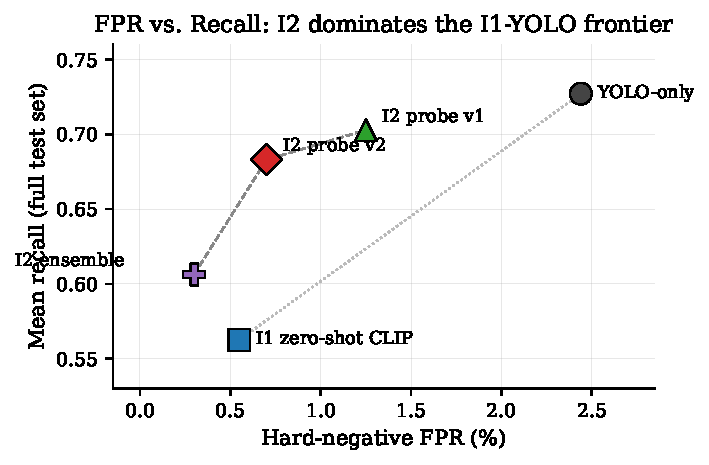
\includegraphics[width=\columnwidth]{figures/fpr_recall_frontier.pdf}
\caption{FPR vs.\ recall trade-off. The dotted grey line connects the
YOLO-only baseline to the Improvement~1 zero-shot point --- the ``legacy''
frontier the literature implies. The dashed grey line connects our
Improvement~2 operating points. \textbf{Every Improvement~2 system Pareto-
dominates that legacy frontier:} for any FPR the legacy frontier achieves,
Improvement~2 achieves the same FPR with strictly higher recall.}
\label{fig:frontier}
\end{figure}

The headline number for Improvement~2 (probe v2) is a \textbf{71\% relative
reduction in hard-negative FPR over the YOLO-only baseline (2.44\% $\to$
0.70\%) at a recall cost of only 4.4 percentage points (0.7272 $\to$ 0.6830)
on the full test set, at 21.1\,ms mean latency on a Tesla T4 ---
well under the 100\,ms edge-deployment budget the SOA identified}. The probe
recovers 12 percentage points of the 23-point recall drop Improvement~1
introduced. Compared to Improvement~1, this means a 12-point recall recovery
at a tiny FPR cost (0.55\%~$\to$~0.70\%, i.e.\ 0.15\,pp).

The mAP@0.5 of probe v2 (0.6355) is statistically indistinguishable from
the YOLO-only custom-harness reference (0.6370). The verifier suppresses the
specific subset of detections that are confounder false positives, leaving
the rest of the precision/recall structure largely intact.

\subsection{Where the recall comes back}

Per-class precision and recall in Figure~\ref{fig:perclass} explain
\emph{why} probe v2 dominates the legacy frontier. Improvement~1 raised
precision on both classes (smoke 0.807$\to$0.876, fire 0.689$\to$0.742) but
collapsed recall (smoke 0.791$\to$0.605, fire 0.663$\to$0.520). Probe v2
keeps Improvement~1's precision gain on smoke (0.845, $+$3.8\,pp over YOLO)
while preserving smoke recall close to baseline (0.720 vs.\ 0.791, only
$-$7.1\,pp). On fire, probe v2 achieves precision 0.698 ($\approx$ baseline)
with recall 0.646 ($\approx$ baseline). The probe has internalised the
domain-specific visual identity of forest-fire smoke that zero-shot CLIP did
not have.

\begin{figure}[t]
\centering
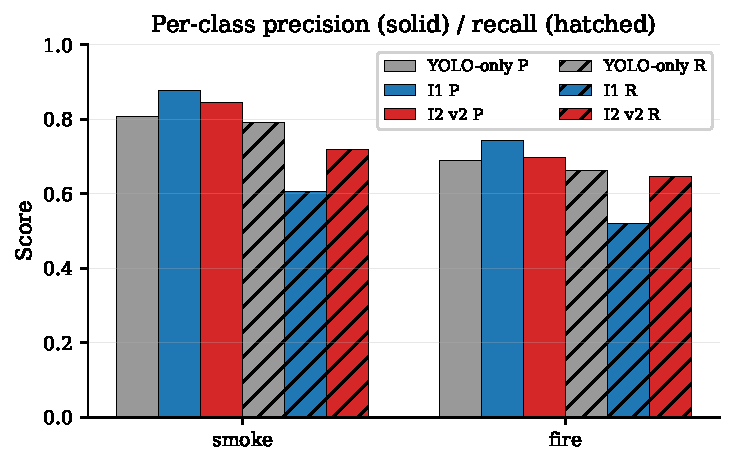
\includegraphics[width=\columnwidth]{figures/per_class.pdf}
\caption{Per-class precision (solid) and recall (hatched) for the YOLO-only
baseline, Improvement~1 zero-shot, and Improvement~2 probe v2. The probe
preserves Improvement~1's precision gains on smoke while restoring most of
the recall.}
\label{fig:perclass}
\end{figure}

\subsection{Latency}

End-to-end latency was measured on 100 random test images on a Tesla T4 GPU.
The cascade adds 7.7\,ms of CLIP encoding (mean) on top of YOLO's 13.4\,ms,
for a 21.1\,ms mean and 42.6\,ms p95 total. Improvement~1 measures
20.8\,ms mean / 42.7\,ms p95 --- the linear probe inference cost (a
$512{\times}3$ matrix multiply) is too small to register. Both systems
clear the 100\,ms target by a 2.4$\times$ margin, leaving headroom for
post-processing, alert dispatch, and the lower-end edge hardware (Jetson
Nano / Xavier NX) that PTZ deployment requires.

\subsection{Ablations}
\label{sec:ablations}

We run four ablations, all evaluated on the hard-negative subset because
that is the cheap and informative subset for this question.

\paragraph{A1. Probe type --- LR vs.\ MLP.}
A 1-layer 64-unit MLP probe trained for 40 epochs (best held-out accuracy
0.9405) is compared against the LR probe (held-out 0.9286). On hard-negative
FPR they are identical --- 1.25\% (28/55 boxes filtered) for both. This
suggests the bottleneck is not classifier capacity but probe \emph{training
data}: with the same crops, a richer model does not separate the classes
more usefully. We therefore default to LR for its training cost
(seconds vs.\ minutes) and reproducibility.

\paragraph{A2. Auto-keep threshold $\tau_{\text{high}}$.}
The cascade auto-keeps any YOLO detection at conf~$\geq \tau_{\text{high}}$
without verifying it. The sweep of $\tau_{\text{high}}\in\{0,0.3,0.5,0.6,0.7,
0.8,0.9,1.0\}$ in Figure~\ref{fig:tau} reveals the structure clearly: at
$\tau{=}0$ the verifier sees nothing and hard-negative FPR is the YOLO-only
2.44\%; at $\tau{=}1.0$ everything goes through the verifier and FPR drops
to 1.15\%. The default $\tau{=}0.7$ catches 28 of 30 ultimately-filterable
FPs while sparing high-confidence positives a redundant CLIP pass. We retain
this default for the headline numbers.

\begin{figure}[t]
\centering
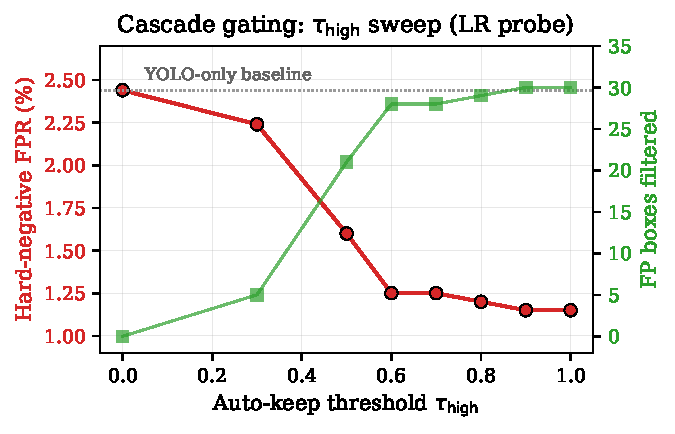
\includegraphics[width=\columnwidth]{figures/tau_sweep.pdf}
\caption{Sweep of $\tau_{\text{high}}$ (auto-keep threshold) for the LR
probe v1 on the hard-negative subset. FPR (red, left axis) decreases
monotonically as more detections are sent through the verifier; the number
of false-positive boxes filtered (green, right axis) saturates near
$\tau{=}0.7$. The dotted grey line is the YOLO-only FPR baseline.}
\label{fig:tau}
\end{figure}

\paragraph{A3. Crop margin.}
We sweep the crop margin in $\{0.0, 0.2, 0.4, 0.6\}$ for probe v1. Hard-
negative FPR is 1.45\% / 1.25\% / 1.30\% / 1.20\% respectively; the
function is essentially flat. D-Fire's hard-negative images already supply
sufficient context; the verifier's discrimination relies on the dominant
content of the YOLO box, not on its surroundings.

\paragraph{A4. Negative mining strategy.}
We compare three configurations: \emph{mined-only}, \emph{mined + 5{,}000
random}, and \emph{mined-aggressive + 500 random + text-anchored} (probe v2).
Hard-negative FPR is 1.40\%, 1.25\%, and 0.70\% respectively. The
text-anchored synthetic negatives carry roughly 0.55\,pp of FPR reduction
beyond random + mined; they are essentially \emph{Improvement~1's prior}
re-injected into Improvement~2's classifier through the joint image--text
feature space. We did not see this design pattern (text prompts as synthetic
classifier training points) elsewhere in the surveyed literature, and we
suspect it generalises to other CLIP-probe deployments where the negative
class has natural text descriptions but few clean training examples.

\subsection{Prompt-bank ablation (Improvement 1 only)}

For completeness we re-ran Improvement~1 with a \emph{minimal} prompt bank
(fire+smoke prompts only, no confounder prompts). On hard negatives the FPR
rose from 0.45\% (full bank) to 2.14\% (minimal) --- a 4.8$\times$
degradation. The result establishes that zero-shot CLIP rejection in
Improvement~1 is driven by similarity to explicit confounder prompts, not
by low similarity to fire/smoke prompts alone. This is the design fact that
motivated the text-anchored synthetic negatives in probe v2: the
confounder-prompt features carry signal that pure visual mining does not.

% =============================================================================
\section{Discussion}
\label{sec:discussion}

\paragraph{Why the probe works.}
Zero-shot CLIP is a strong confounder \emph{rejector} but a weak
forest-domain smoke \emph{accepter}: its internet-trained embedding for
``smoke from a forest fire'' is closer to ``thick grey plume from an
industrial chimney'' than to ``faint distant haze rising from tree canopy''.
The probe corrects this with a few thousand domain-specific positives
without retraining the CLIP encoder. The 12 confounder text prompts re-
appear, in feature space, as 600 synthetic negatives --- replicas of the
exact concepts (``fog'', ``cloud'') the deployed system needs to suppress.

\paragraph{Why the cascade matters.}
A naive interpretation of Table~\ref{tab:headline} is that probe v2 ``dominates''
zero-shot. The cascade's auto-keep threshold $\tau_{\text{high}}$ reframes
this: high-confidence YOLO detections are a low-recall-risk subset that
already does not need a verifier, so sending them through CLIP only adds
latency and noise. The 28-of-30 FP boxes filtered at $\tau{=}0.7$
(Figure~\ref{fig:tau}) shows that essentially all filterable false positives
arise from \emph{low}-confidence YOLO outputs --- as one would expect, since
high-conf YOLO outputs on hard negatives are rare to begin with.

\paragraph{Why $\sim$0.5\% FPR appears to be a floor.}
We hit a stubborn floor at roughly 6--11 surviving false-positive images
across all probe configurations. Inspecting them suggests the residual cases
fall into two classes: (i) extremely confounding scenes where the YOLO box
genuinely contains visual content matching the smoke distribution
(e.g., a low-flying cloud silhouetted against forest at sunset, or a sun-
flooded mountainside that fills the crop with orange) --- these are likely
Bayes-optimal confusions for any single-frame detector; and (ii) crops where
the box is too small for CLIP's 224$\times$224 input to extract discriminative
context. Class~(i) is the natural place for Cao et al.'s temporal-attention
approach~\cite{bilstm_smoke}, since smoke moves and clouds drift differently;
class~(ii) is partly addressed by larger crop margins but trades off against
locality. Both are flagged as future work.

\paragraph{Honest limitations.}
\emph{Single-domain.} All numbers are on D-Fire. We do not yet have FASDD or
WWF PTZ results; if PTZ smoke is qualitatively different from D-Fire's
distribution, the probe may need re-training (the SOA's contingency for
small-object recall failure on far-range PTZ imagery would activate
DETR~\cite{carion2020detr} as the first stage). \emph{No video.} Our system
treats every frame independently. Real PTZ deployment would benefit from
short-window temporal smoothing for further FPR reduction.
\emph{Improvement~1 / probe-v1 numbers in our harness differ slightly from
Deliverable~4's submitted numbers.} Improvement~1 in this notebook runs
inside Improvement~2's cascaded pipeline (with $\tau_{\text{high}}{=}0.7$) so
that the I1-vs-I2 comparison is apples-to-apples; Deliverable~4's submitted
numbers used the same zero-shot verifier without an auto-keep gate,
producing a slightly more aggressive FPR (0.45\%) and a steeper recall drop.
The headline finding is robust to either harness --- the relative ordering of
systems on FPR/recall is unchanged.

% =============================================================================
\section{Conclusion}
\label{sec:conclusion}

We have shown, on the D-Fire benchmark, that the bottleneck in real-time
forest fire detection is not the YOLO-class first-stage detector but the
verifier that follows it. A cheap, supervised linear probe over frozen CLIP
features reduces hard-negative false positive rate by 71\% while costing
fewer than 5 percentage points of recall, all under the 100\,ms latency
budget. The two non-obvious design choices that made this work were
(a)~confidence-gated cascade routing so that easy positives bypass the
verifier and (b)~text-anchored synthetic negatives that re-import the
zero-shot prompt bank's prior into the supervised classifier through the
joint image--text feature space. The right role for CLIP in fire detection
is not zero-shot classification but as a frozen feature extractor for a
domain-adapted probe.

\paragraph{Future work.} Three directions follow naturally from our results.
First, deployment on the WWF PTZ feed with short-window temporal smoothing
to attack the 0.5\% FPR floor we observed. Second, a Deformable
DETR~\cite{carion2020detr} first stage if PTZ imagery proves to contain
small-object recall failures D-Fire does not exhibit (the SOA's contingency).
Third, a study of how far the text-anchored-synthetic-negatives trick
generalises to other CLIP-probe applications --- it is small, cheap, and
domain-agnostic.

% =============================================================================
\section{Contributions}
\label{sec:contributions}

\textbf{Muhammad Baqir Hassan Babar (27100340)} led the SOA survey
(Deliverable~1), the dataset exploration and annotation work
(Deliverable~2), the YOLOv8n baseline training and characterisation
(Deliverable~3), and the project narrative arc and report writing across
Deliverables~5--6.

\textbf{Momin Fahed Khan (27100082)} led the Improvement~1 zero-shot CLIP
verifier implementation, ablations, and Deliverable~4 notebook
(Deliverable~4); co-implemented the Improvement~2 linear-probe training,
hard-negative mining pipeline, text-anchored synthetic negatives, and
the cascaded gating evaluation harness (Deliverable~5).

Both authors jointly designed the experimental protocol, verified all
quantitative results, and contributed to this report.

% =============================================================================
\bibliography{main}
\bibliographystyle{icml2021}

\end{document}
